% -%-%-%-%-%-%-%-%-%-%-%-%-%-%-%-%-%-%-%-%-%-%-%-%-%
% MDI224 % 
% Data:12/12/2011                                 %
% Paris,France                                    % 
% Groupe:                                         %
% - Tiago Chedraoui Silva                   % 
% - Anthony CLERBOUT
% -%-%-%-%-%-%-%-%-%-%-%-%-%-%-%-%-%-%-%-%-%-%-%-%-%

\documentclass[a4paper,11pt]{article}

\usepackage[francais,listings,algo]{tcs}

% Cover %
\def \ttprofname{Roland BADEAU} % teachers name
\def \ttabrv{MDI224} % abbreviation of names class
\def \ttabrvxt{} % period
\def \mytitle{Interpolation par splines cubiques} % Big title
\def \mysubtitle{ Travaux Pratique 1 - Deuxième semestre de 2011} % subtitle
\def \ttauthi{Anthony CLERBOUT} % author's name
\def \ttxti{Casier: 234} % Extra text right side of name
\def \ttauthii{Tiago CHEDRAUOI SILVA} % author's name
\def \ttxtii{Casier: 214 } % Extra text right side of name
\def \ttdate{Décembre 15, 2011} % date

\begin{document}
\titleTMB 
\newpage
\tableofcontents
\listoffigures
\newpage

\section{Résolution du système linéaire}

\subsection{Méthode de Jacobi}
Jacobi converge ssi $\rho(D-1(L+U)) < 1$ d'après le cours.
Or ici, $max (L) = max (U) = 1$ et $D-1$ est une matrice diagonale dont la plus grande valeur propre est $\frac{1}{2}$.
Donc $\rho < 1$.

\subsubsection{Implémentation}

Pour voir la méthode de Jacobi, on a fait le code suivant:

\begin{multicols}{2}
  \lstinputlisting[title=\textbf{Méthode de Jacobi}]{../jacobi.m}
\end{multicols}

\newpage

Pour  voir le  convergence  de la  méthode de  Jacobi,  on a  pris, pour  chaque
itération, chaque valeur de x
calculée jusqu'au moment oú le critére d`arrêt est atteint. Après, on a fait la comparaison de
chaque x avec la valeur optimale (xex) en prenant le log de la différence:

\subsubsection{Convergence}
\begin{figure}[h!]
  \begin{centering}
    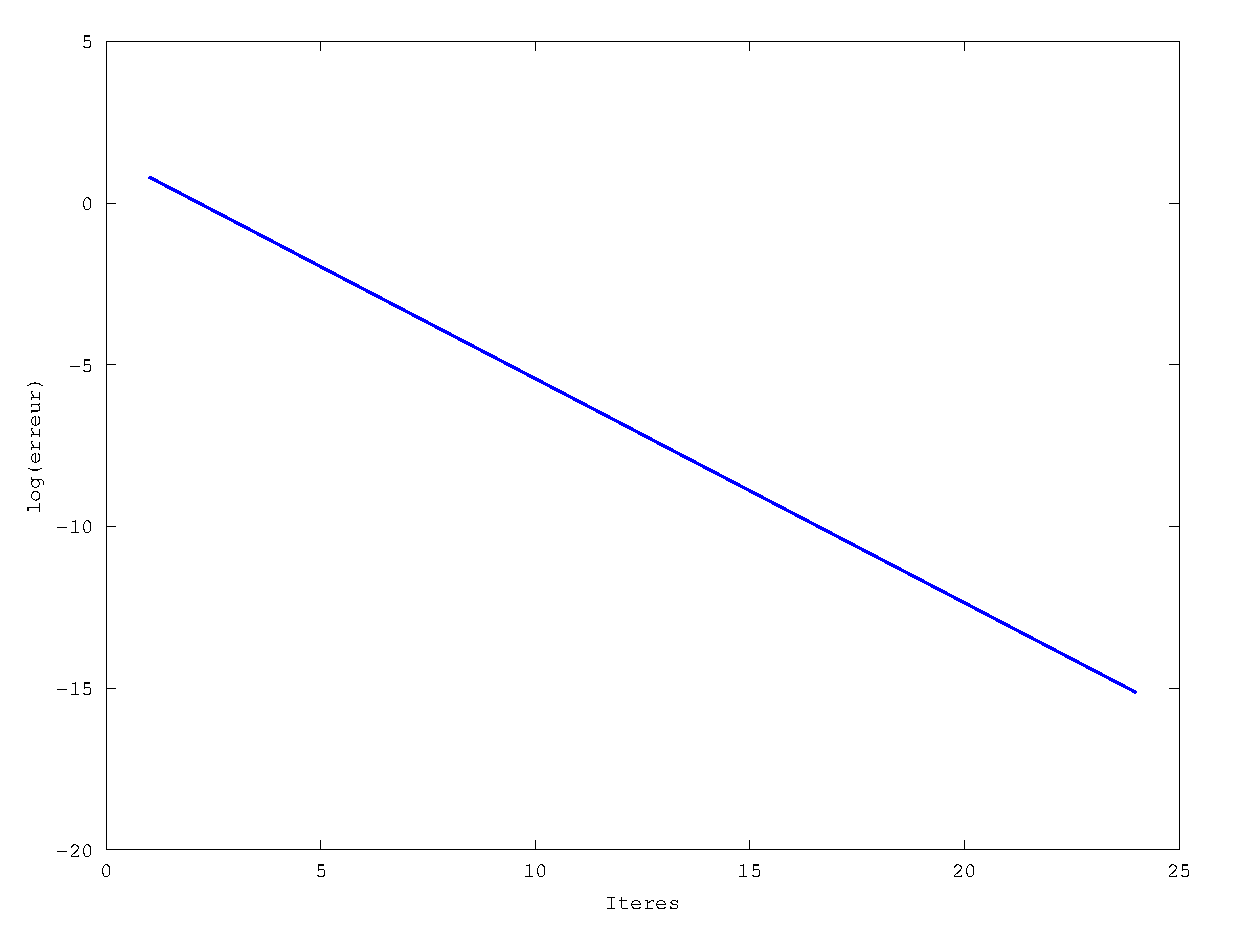
\includegraphics[scale=0.5]{../jacobi_graph}
    \label{rspro2}
    \par\end{centering}
  \caption{Convergence de la méthode de Jacobi}
  \label{fig:jacobi-conv}
\end{figure}

En utilisant la fonction polyfit, nous avons trouvé le polynome: 
$p(x)= -0.693147 x + 1.497866  $


\subsection{Méthode de relaxation}

La çéthode de la relaxation converge ssi $(\frac{D}{w}-L)-(\frac{(1-w)}{w} D + U) <1$ d'après le
cours si A est tridiagonale et définie positive, alors la suite $(x_k)$ converge effectivement vers l'unique solution de $Ax=b$.

\subsubsection{Implémentation}
Pour voir la méthode SOR (relaxation), on a fait le code suivant:

\begin{multicols}{2}
  \lstinputlisting[title=\textbf{Méthode de Relaxation}]{../relax.m}
\end{multicols}

Pour voir la convergence de la méthode SOR, on a pris, pour chaque
itération, chaque valeur de x
calculée jusqu'au moment l'algorithme atteint son critére d'arrêt( pour w=1.0). Après, on a fait la comparaison de
chaque x avec la valeur optimal (xex) en prenant le log de la différence:


\subsubsection{Convergence}
\begin{figure}[h!]
  \begin{centering}
    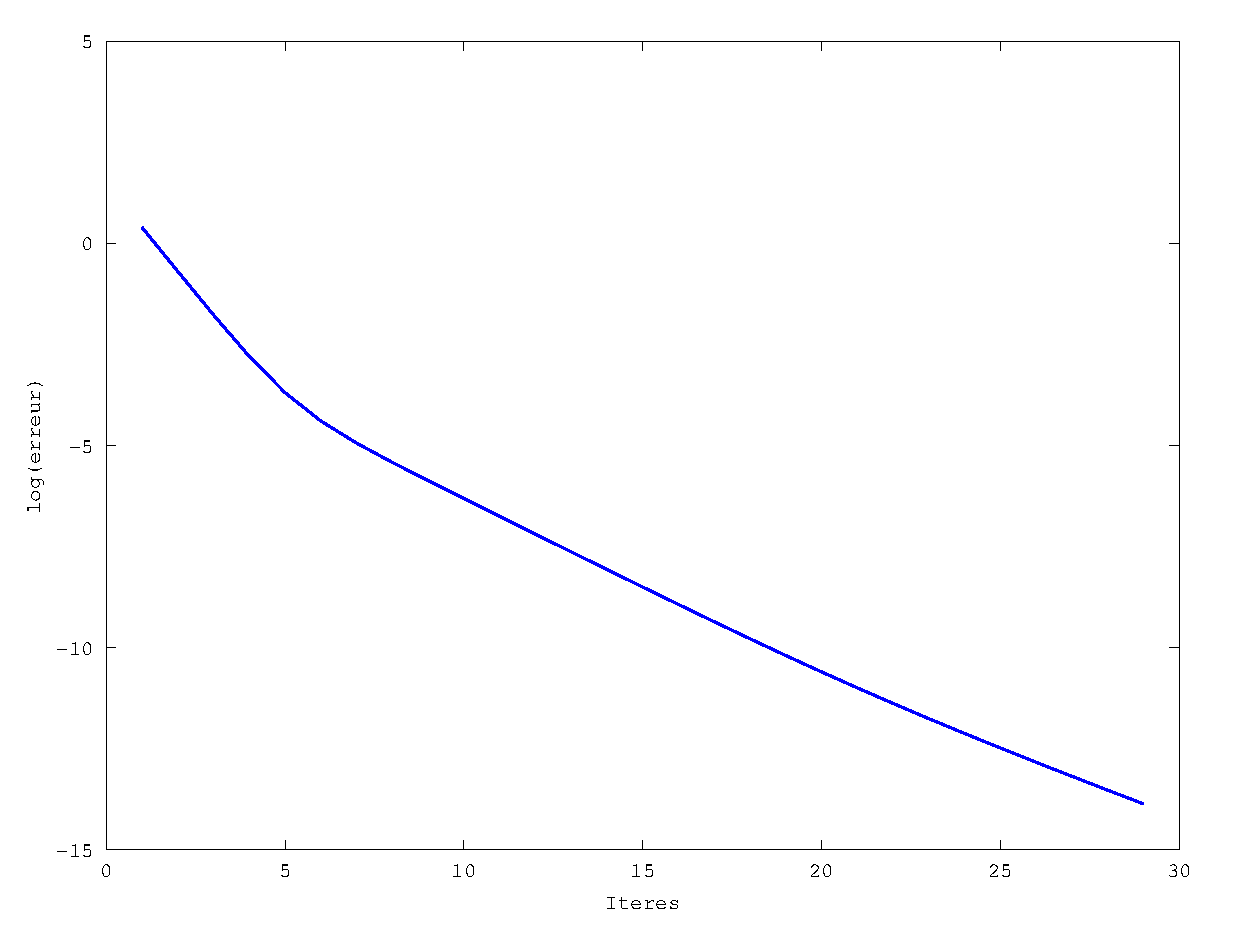
\includegraphics[scale=0.5]{../relaxation_graph}
    \label{rspro2}
    \par\end{centering}
  \caption{Convergence de la méthode de Relaxation pour w=1.0}
  \label{fig:jacobi-conv}
\end{figure}




Pour voir le taux, il existe deux méthodes.
La première utilise les erreurs
et la fonction polyfit de matlab. 
La deuxième le rayon spectral de la
matrice $R_w$. 
Ainsi,  on change  les valeurs  de $w$  de manière  à trouver le
meilleur taux de convergence. Les graphes  pour les deux approches sont représentés dans
les graphes en 3 et 4 bas.
On a trouvé un $w_{optimal}\approx 1.1$ 


\begin{figure}[h!]
  \begin{centering}
    \subfigure[Utilisant la fonction Polyfit et la suite d'erreurs]{
      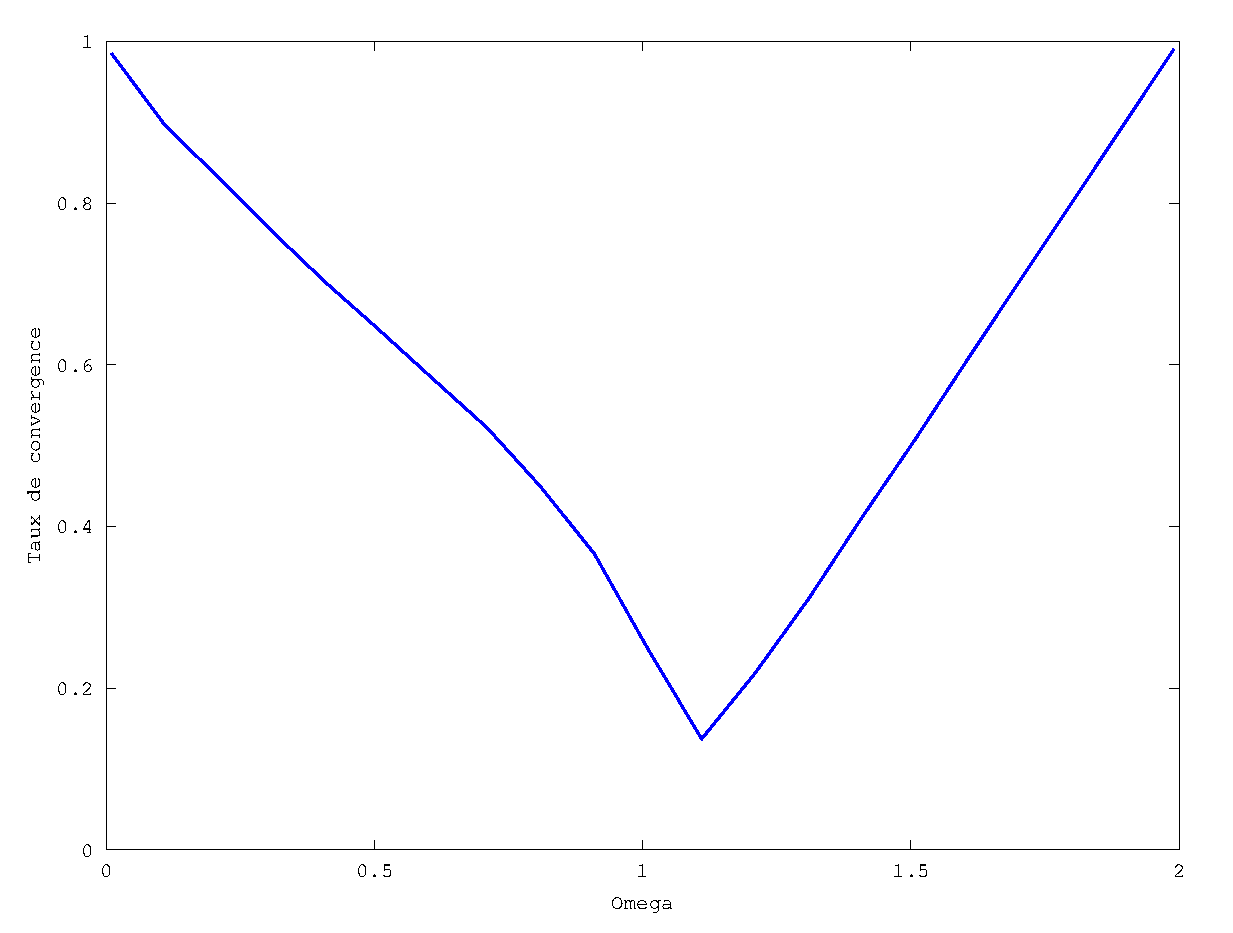
\includegraphics[scale=0.35]{../relaxation_conv2}}  
    \subfigure[Calcule du rayon spectral de la matrice $R_w$.]{
      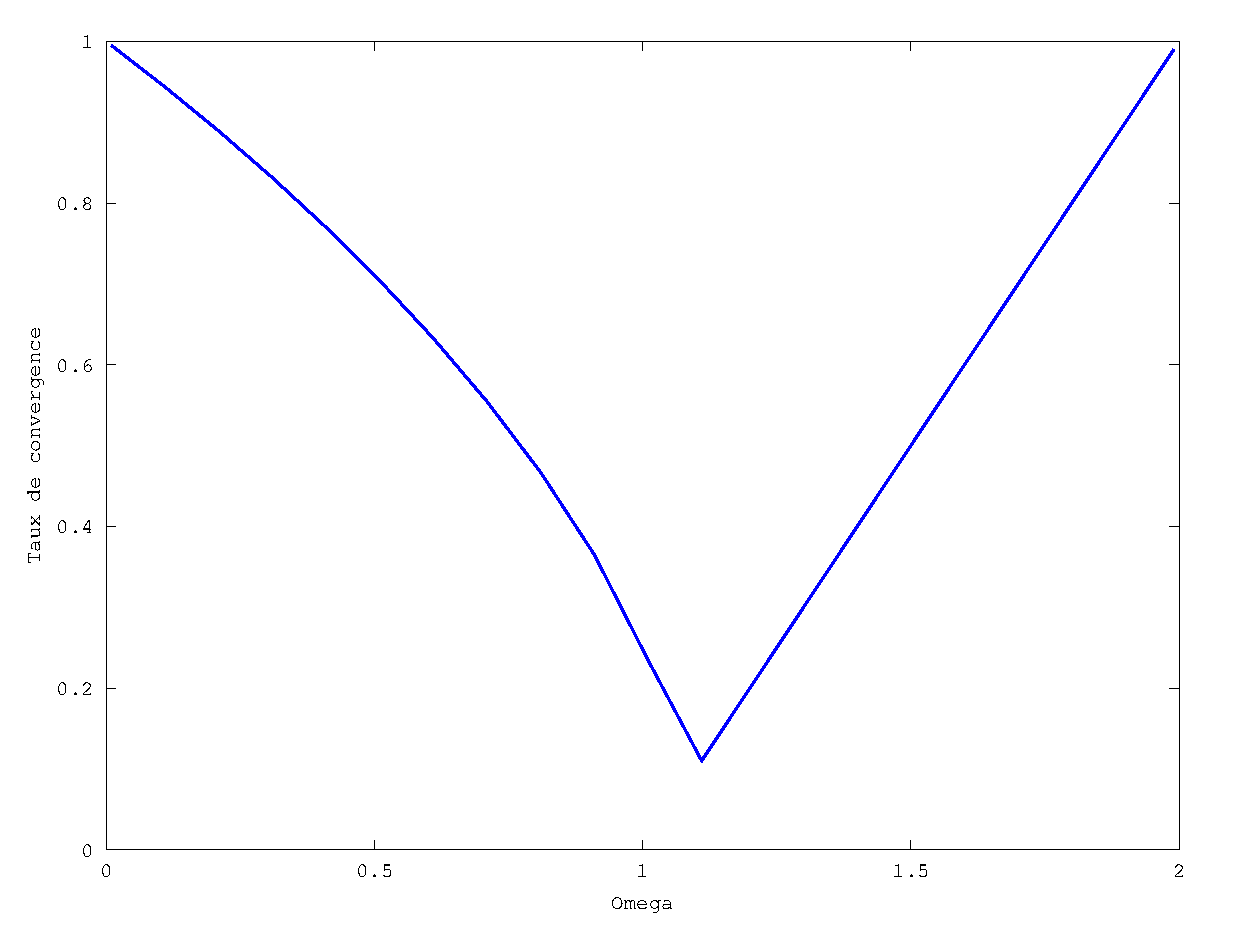
\includegraphics[scale=0.35]{../relaxation_conv_rho}
    }
    \par\end{centering}
  \caption{Taux de convergence en fonction du paramètre de relaxation $\omega$}
  \label{rspro}
\end{figure}


% \begin{figure}[h!]
%   \begin{centering}
%     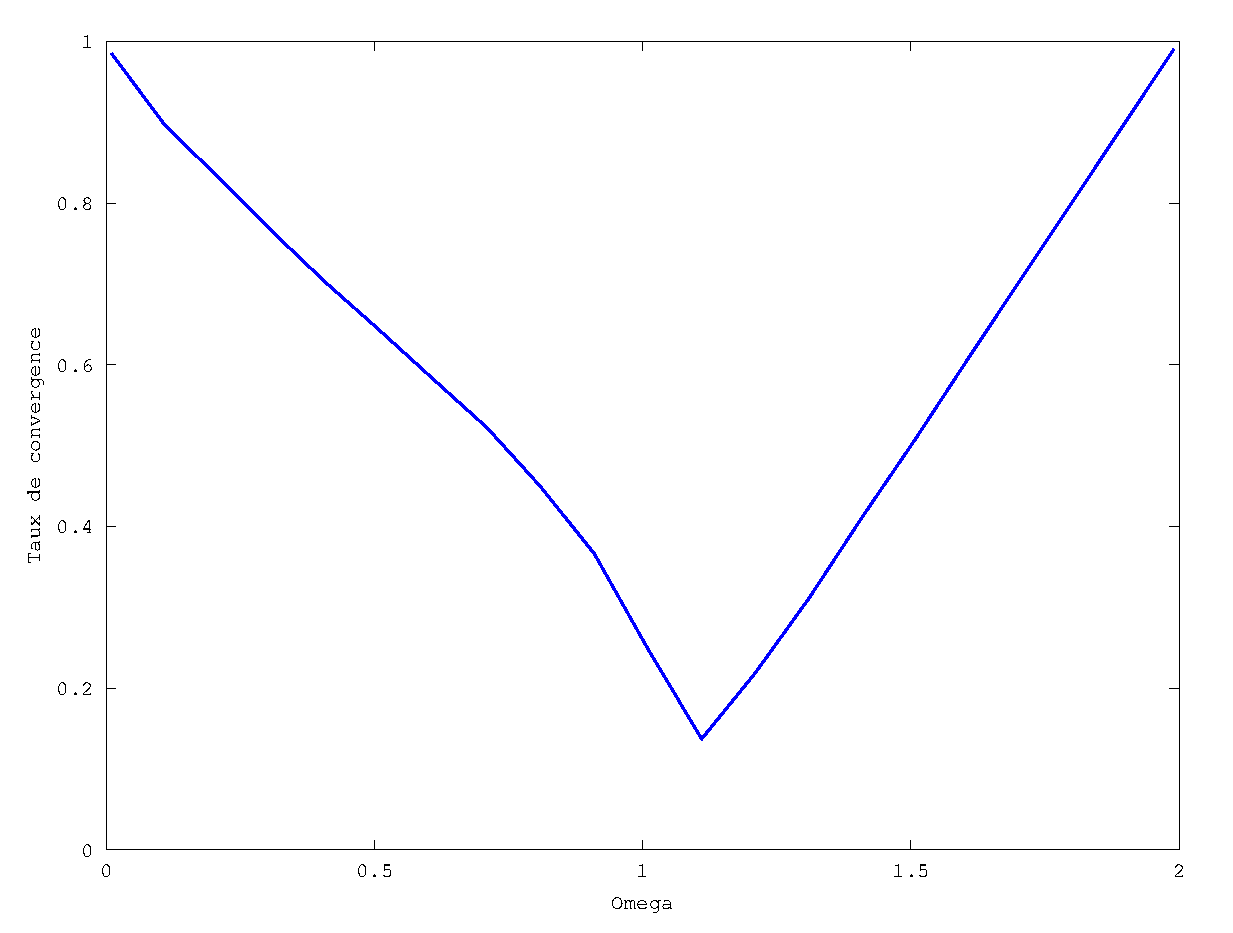
\includegraphics[scale=0.5]{../relaxation_conv2}
%     \label{rspro2}
%     \par\end{centering}
%   \caption{Approche 1:Taux de convergence en fonction du paramètre de relaxation w}
%   \label{fig:jacobi-conv}
% \end{figure}

% \begin{figure}[h!]
%   \begin{centering}
%     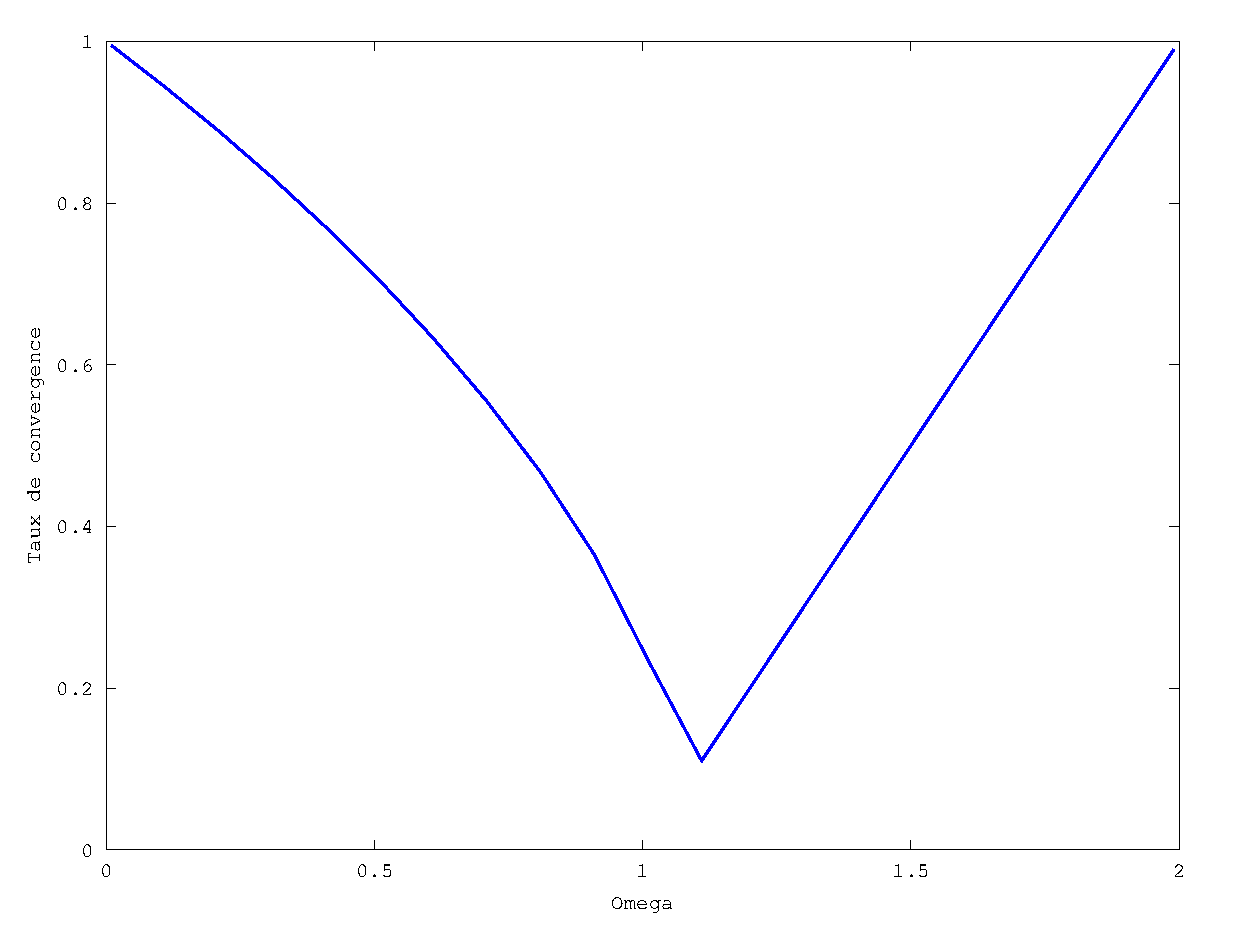
\includegraphics[scale=0.5]{../relaxation_conv_rho}
%     \label{rspro2}
%     \par\end{centering}
%   \caption{Approche 2: Calcul du rayon spectral de la matrice $R_w$}
%   \label{fig:jacobi-conv}
% \end{figure}

%\begin{equation}
%  \omega = \frac{2}{1+\sqrt{1- \rho(J)^2}}
%\end{equation}

%\begin{equation}
%  \frac{d\omega}{d\rho} =\frac{2\,\rho}{\sqrt{1-{\rho}^{2}}\,{\left( \sqrt{1-{\rho}^{2}}+1\right) }^{2}}
%\end{equation}

%Pour la valeur minimale ou maximale, la dérivée doit être 0, donc $\rho(J)=0$,
%en utilisant l'équation 1 on a $\omega=1$;

\newpage
\subsection{Méthode de Cholesky}
\subsubsection{Implémentation}

La fonction suivante était fournie par le problème. 
\begin{multicols}{2}
  \lstinputlisting[title=\textbf{Méthode de Cholesky}]{../cholesky.m}
\end{multicols}

Pour le même exemple que précèdemmet, on a trouvé:

\begin{table}[h!]
  \begin{center}
    \begin{tabular}{|c|c|}
      \hline 
      p & x \\
      \hline 
      \hline 
      4 & [ 1.00000;1.00000;1.00000;1.00000;1.00000]\\
      3 & [ 1.00000;1.00000;1.00000;1.00000;1.00000]\\
      2 & [ 1.00000;1.00000;1.00000;1.00000;1.00000]\\
      1 & [ 1.00000;1.00000;1.00000;1.00000;1.00000]\\
      \hline 
    \end{tabular}
  \end{center}
  \caption{Vérification fonction Cholesky}
\end{table}

\subsubsection{Complexité}

La complexité de la fonction Cholesky est donnée par $O(\frac{N^2p}{2})$, pour les autres
méthodes on a:

\begin{description}
\item[Jacobi]{Le calcul de $x^{n+1}$ par Jacobi est donné  par: $x^{n+1}=D^{-1}(L+U)x^n +
  D^{-1}b$. Comme la  matrice  A   est composée seulement de termes  non  nuls dans  la
  diagonale principale et dans deux diagonales secondaires, on a: $(L+U)$ qui est une matrice
  avec environ 2N termes et  $(D)^{-1}$ est une matrice avec  N termes : 

Ainsi,  le  nombre  de  multiplications pour calculer $D^{-1}(L+U)x^n  \in  O(3N)$. De plus, $D^{-1}b
  \in O(N)$}, que l'on peut donc négliger. Finalement, $Jacobi \in O(3N)$
 
\item[Relaxation]{'Le calcul de  $x^{n+1}$ par la méthode de la Relaxation est donné  par: $x^{n+1}=(\frac{D}{w}-L)^{-1}(\frac{1-w}{w}D+U)x^n +  (\frac{D}{w}-L)^{-1}b$ . Comme la matrice A est composée seulement par des termes non nuls dans la
  diagonale   principale   et   dans   deux   diagonales   secondaires,   on   a:
  $(\frac{D}{w}-L)^{-1} $ qui est une matrice avec plus de $2N$ termes (on a trouvé cette valeur en
  utilisant Matlab pour la matrice A dans la section précédente)
         et $(\frac{1-w}{w}D+U)$ est alors une matrice avec 2N termes. Ainsi,
  $(\frac{D}{w}-L)^{-1}(\frac{1-w}{w}D+U)x^n         \in        O(5N)$        et
  $(\frac{D}{w}-L)^{-1}b \in O(3N)$. Finalement $Relax \in O(5N)$
}
\end{description}

Afin de calculer le temps d'exécution des méthodes de Jacobi, Relaxation et
Cholesky, les codes suivants ont été crées.


\begin{multicols}{2}
  \lstinputlisting[title=\textbf{Calcul temps Jacobi}]{time/entreeJacobi.m}
\end{multicols}

\begin{multicols}{2}
  \lstinputlisting[title=\textbf{Calcul temps Relaxation}]{time/entreeRelax.m}
\end{multicols}


\begin{multicols}{2}
  \lstinputlisting[title=\textbf{Calcul temps Cholesky}]{time/entreeCholesky.m}
\end{multicols}

En exécutant les codes, on a trouvé:

\begin{table}[h!]
  \begin{center}
    \begin{tabular}{|c|c|c|c|c|c|c|}
      \hline 
      N & 50 & 100 & 150 & 200 & 250 & 300 \\
      \hline 
      \hline 
      Cholesky $(p=1)$ & 0.011554       &  0.023093 & 0.036068
      & 0.047571 & 0.061026 & 0.074059 \\
      Jacobi &   0.0026100
      & 0.0031020
      & 0.0041549
      & 0.0048039
      & 0.0078550
      & 0.0097679        \\
      Relaxation $(w = 1.1)$
      & 0.0020840
      & 0.0025171
      & 0.0036389 
      & 0.0065949
      & 0.0083960
      & 0.018082\\
      \hline 
    \end{tabular}
  \end{center}
  \caption{Comparaison des temps entre les trois méthodes pour un système tridiagonal}
\end{table}

En général la méthode Jacobi est la méthode la plus rapide pour un
système     tridiagonal,    parce     qu'elle    fait     moins  de
multiplications. Néanmoins, la méthode de relaxation fait moins d'itérations que
Jacobi, c'est pour cela que quand N  est petite la méthode relaxation est plus rapide
que Jacobi; mais lorsque N croit beaucoup, la méthode de Jacobi fait moins multiplications
même avec plus d'interaction, ce qui le fait le plus vite.


\section{Application}
\subsection{Calcul d'une spline d'interpolation}
\begin{multicols}{2}
  \lstinputlisting[title=\textbf{Méthode spline cubique}]{../sinterp.m}
\end{multicols}

\subsection{Évaluation d'une fonction spline cubique}


\begin{multicols}{2}
  \lstinputlisting[title=\textbf{Méthode spline cubique}]{../speval.m}
\end{multicols}

\subsection{Application}

En utilisant les fonctions mis en œuvre avant (relax et sinterp), on a utilisé les fonctions sinus
et exponentielle pour vérifier le spline cubique. Les graphes suivants sont les valeurs interpolées par le
spline cubique  et l'erreur de cette  interpolation est la  comparaison entre la
valeur calculée par l 'algorithme et la valeur rélle de la fonction.

 Une observation: les graphes des erreurs montrent que les points d'ordonnée 
 nulle  sont  les points utilisées  pour trouver  les valeurs pendant l'interpolation,
 c'est-à-dire, que ce sont les points en commun entre la fonction
réelle et la valeur de l'interpolation. Donc il n'existe pas d'erreur parce que c'est la même valeur.
Une autre remarque  est que plus la  valeur de la fonction est  grande, plus est
l'erreur est importante.

Pour les graphes 6 et 9, on a  augmenté le valeur du pas de la fonction original,
cela  veut   dire,  on  a  pris   plus  de  points  en   utilisant  la  fonction
original. Alors, la  spline cubique ira être plus précise, comme  on voit par le
graphes des erreurs qui démontrent des valeurs trop petites.

Autre remarque c'est que on a, en utilisant les fonctions spinterp et 
relax, des erreurs avant la fonction speval. Donc, pour avoir une spline plus précise on pourrait aussi
faire des améliorations dans la fonctions relax et spinterp.

\begin{figure}[h!]
  \begin{centering}
    \subfigure[Interpolation]{
      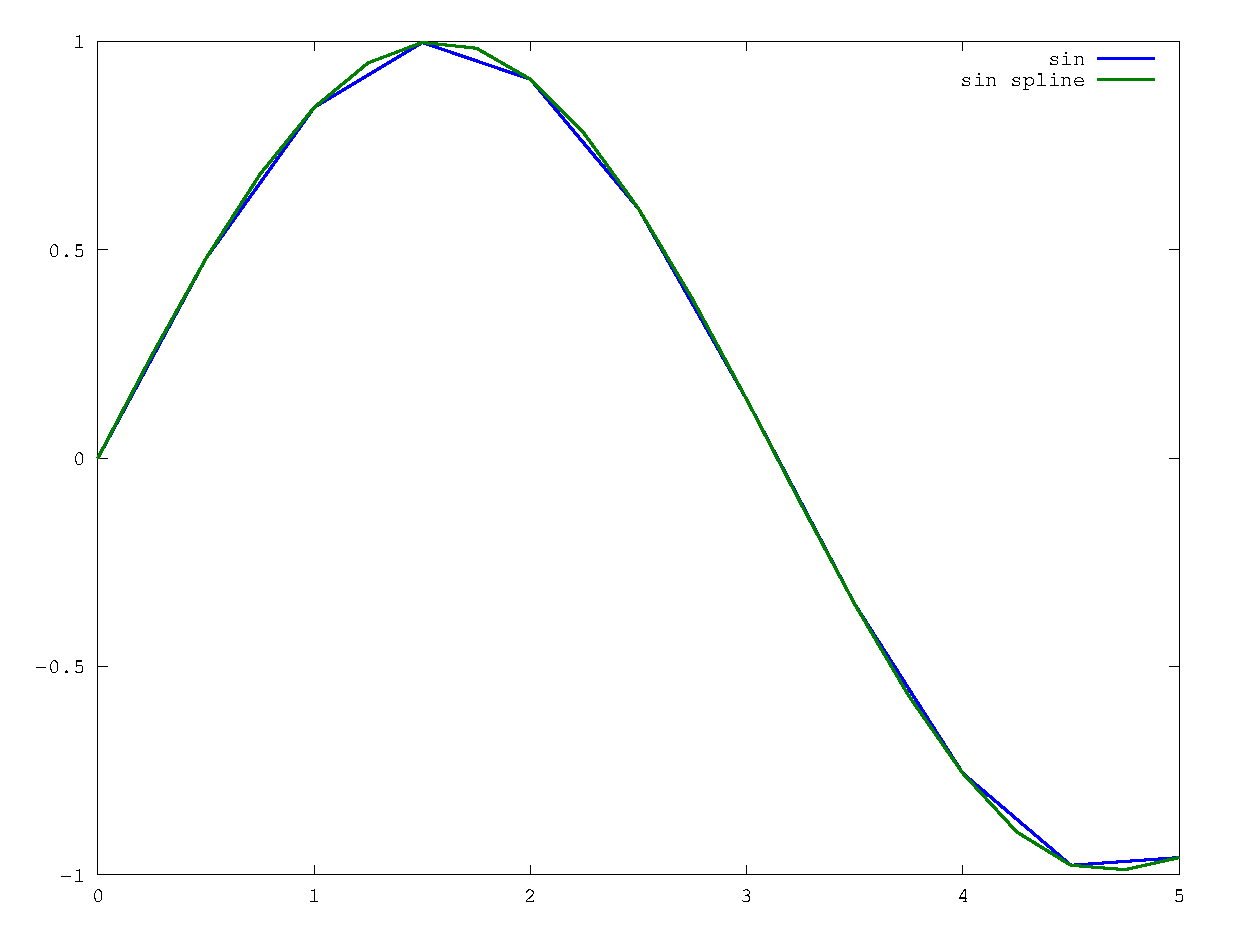
\includegraphics[scale=0.35]{../sinus_2}    }
    \subfigure[Erreur interpolation.]{
      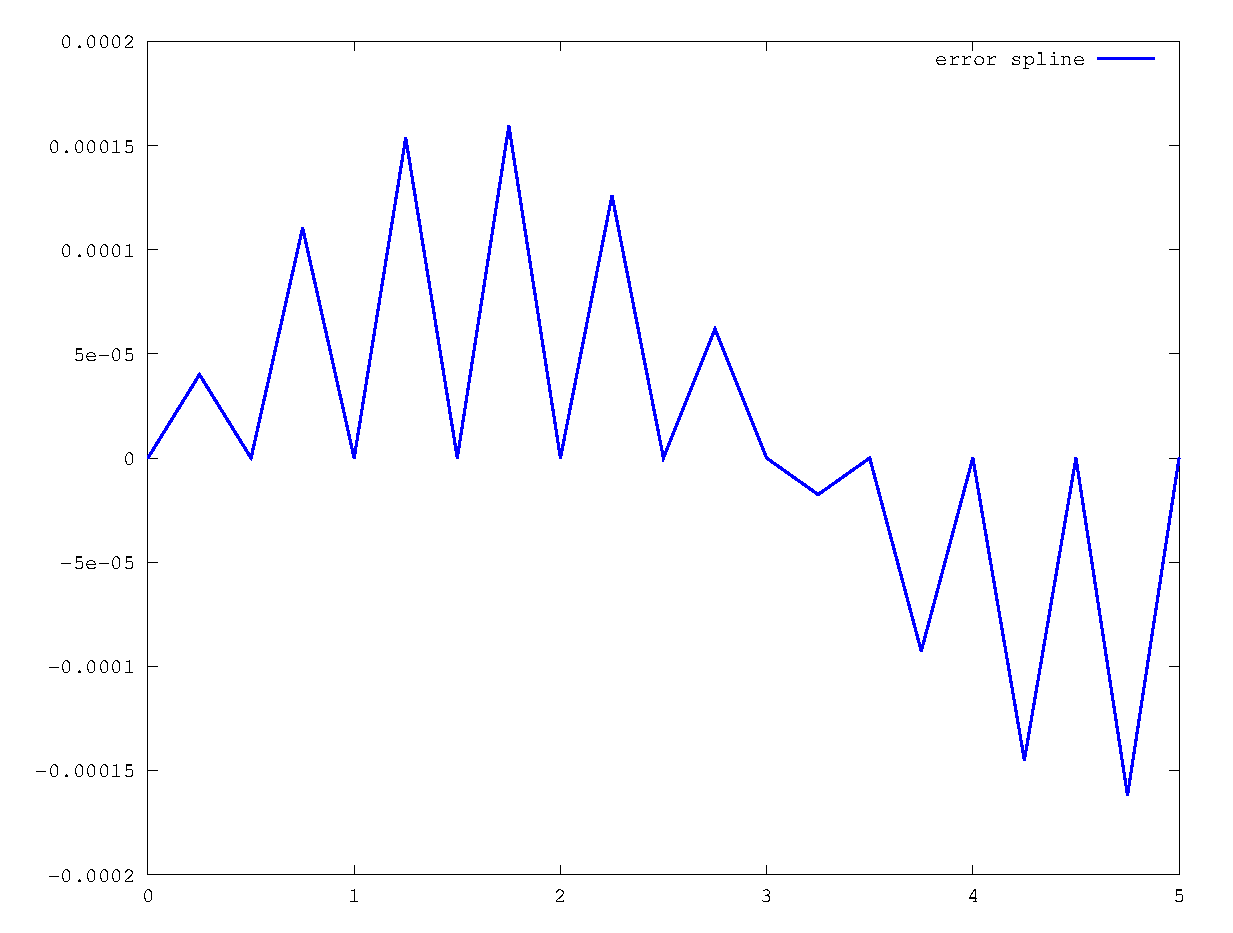
\includegraphics[scale=0.35]{../sinus_2_error}
    }
    \par\end{centering}
  \caption{Fonction sinus pas original 0.5, pas spline 0.25}
\end{figure}


\begin{figure}[h!]
  \begin{centering}
    \subfigure[Interpolation]{
      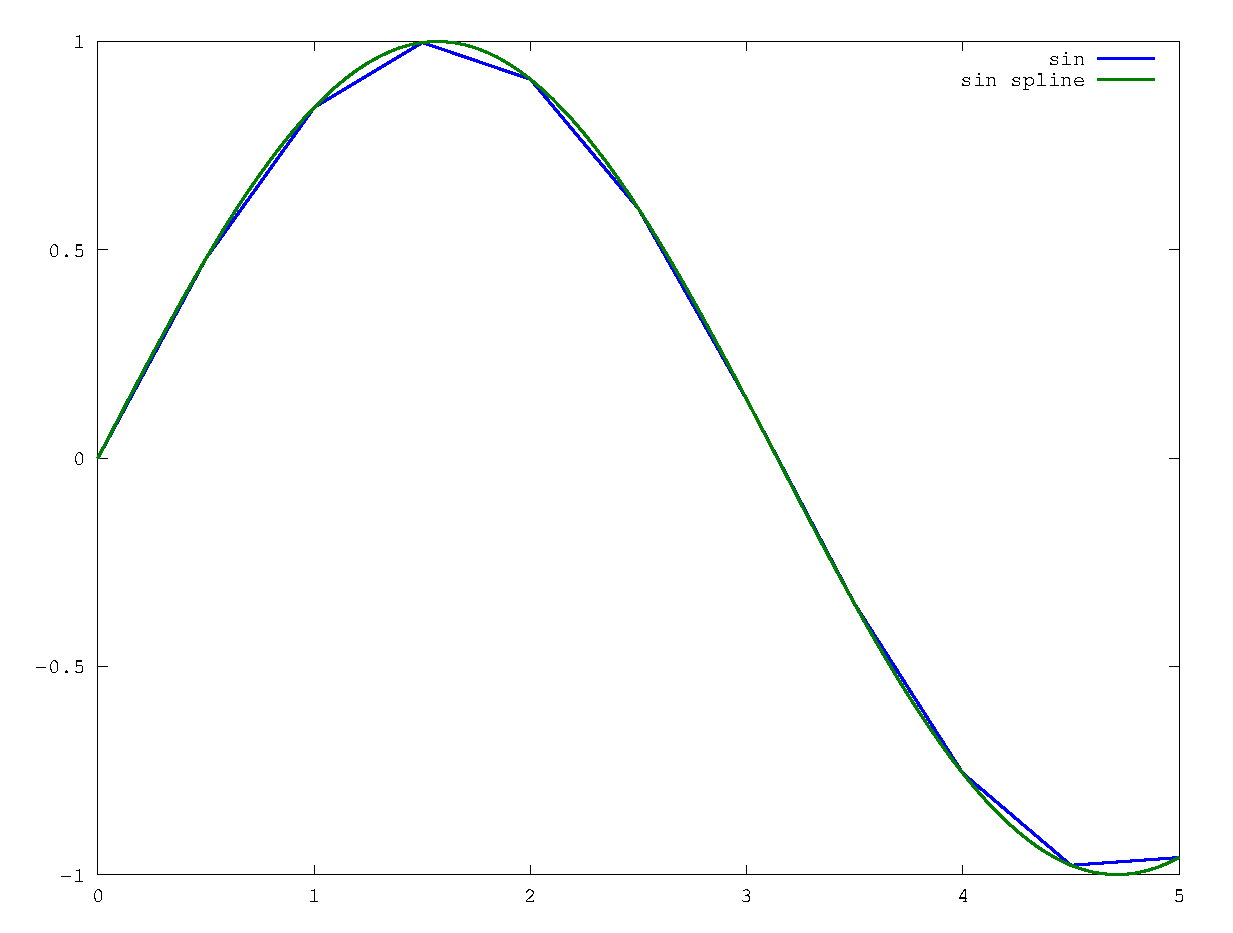
\includegraphics[scale=0.35]{../sinus_10}    }
    \subfigure[Erreur interpolation.]{
      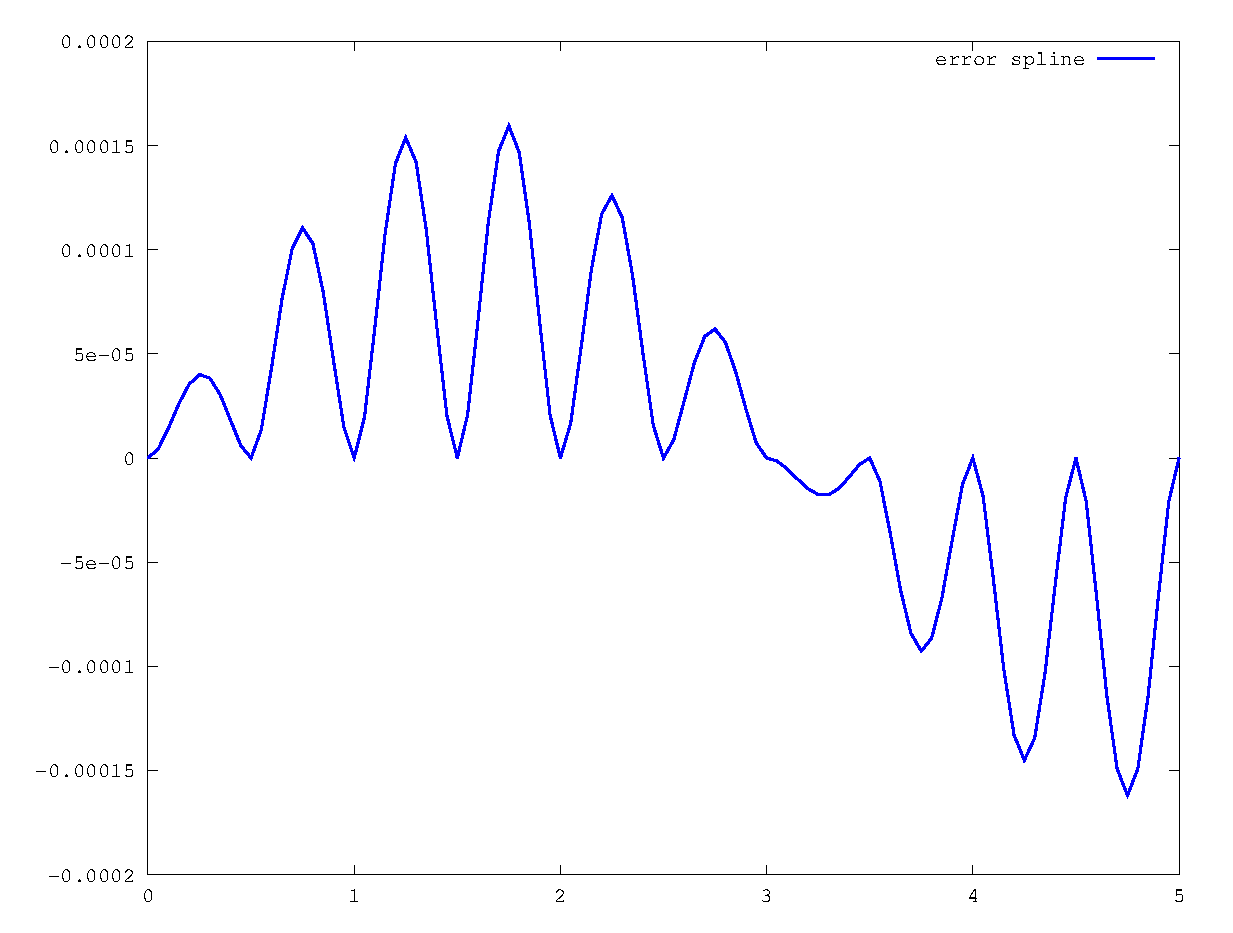
\includegraphics[scale=0.35]{../sinus_10_error}
    }
    \par\end{centering}
  \caption{Fonction sinus pas original 0.5, pas spline 0.05}
\end{figure}


\begin{figure}[h!]
  \begin{centering}
    \subfigure[Interpolation]{
      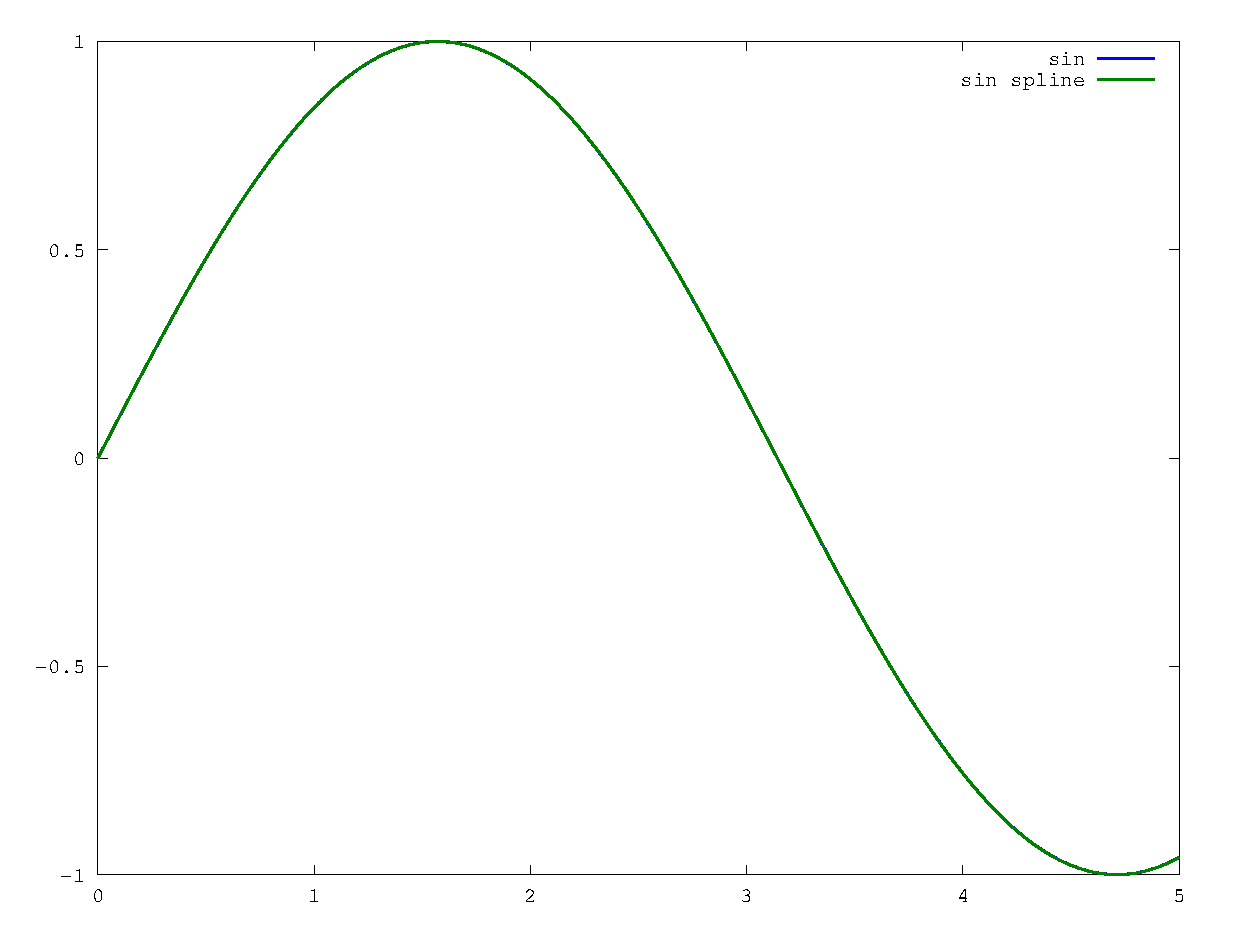
\includegraphics[scale=0.35]{../sinus_10_2}    }
    \subfigure[Erreur interpolation.]{
      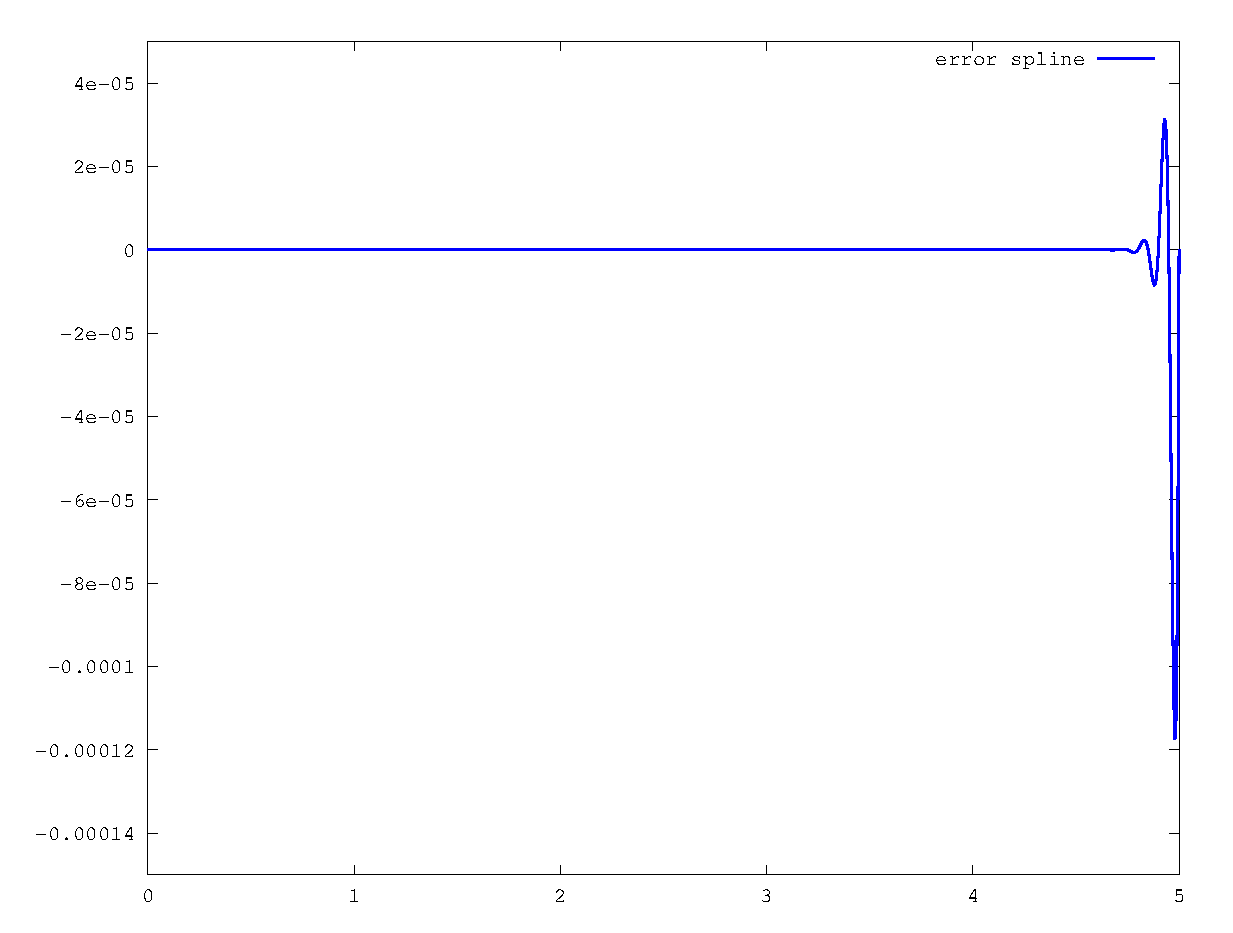
\includegraphics[scale=0.35]{../sinus_10_error_2}
    }
    \par\end{centering}
  \caption{Fonction sinus pas original 0.05, pas spline 0.005}
\end{figure}

\begin{figure}[h!]
  \begin{centering}
    \subfigure[Interpolation]{
      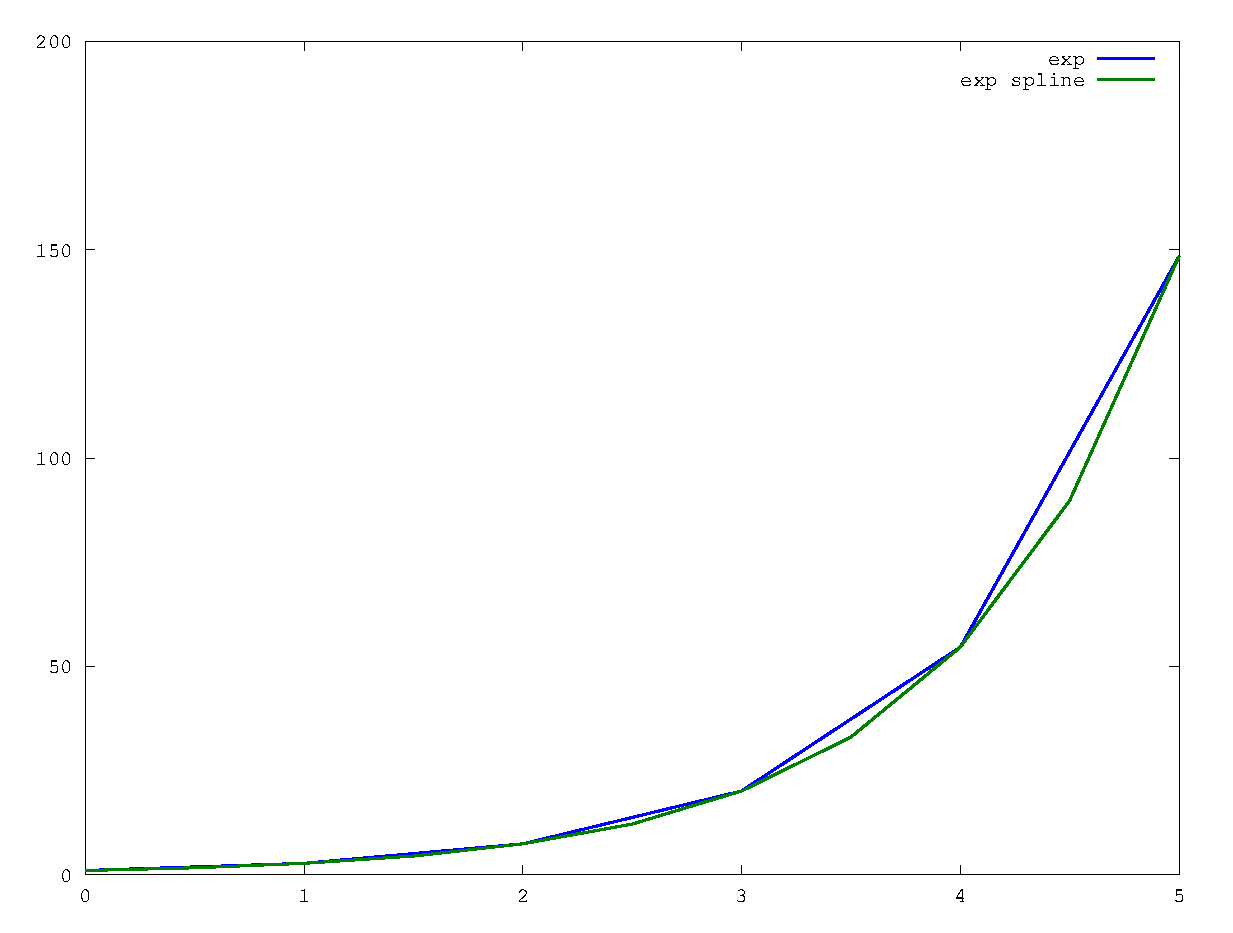
\includegraphics[scale=0.35]{../exp_2}    }
    \subfigure[Erreur interpolation.]{
      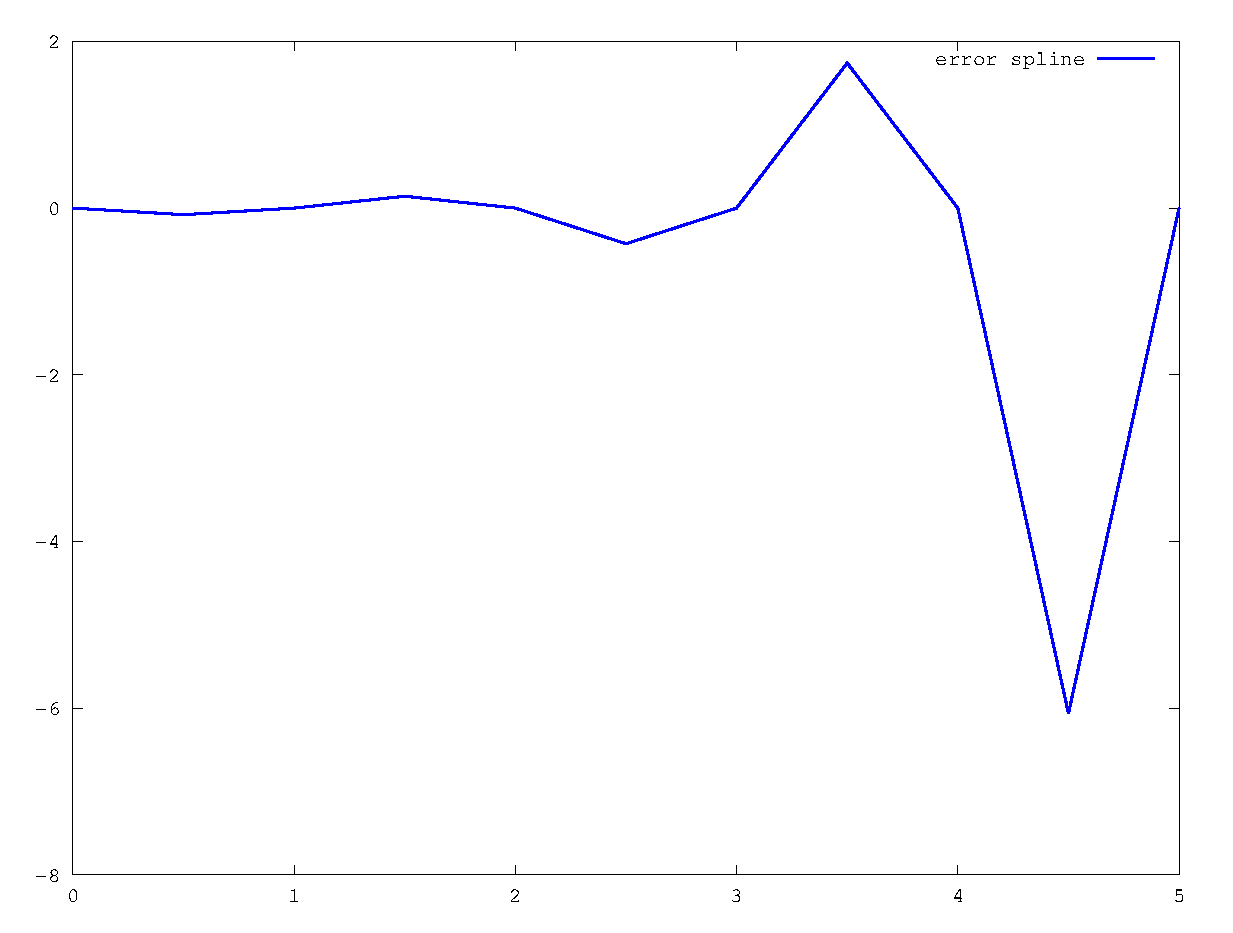
\includegraphics[scale=0.35]{../exp_2_error}
    }
    \par\end{centering}
  \caption{Fonction exp pas original 1, pas spline 0.5}
  \label{rspro}
\end{figure}


\begin{figure}[h!]
  \begin{centering}
    \subfigure[Interpolation]{
      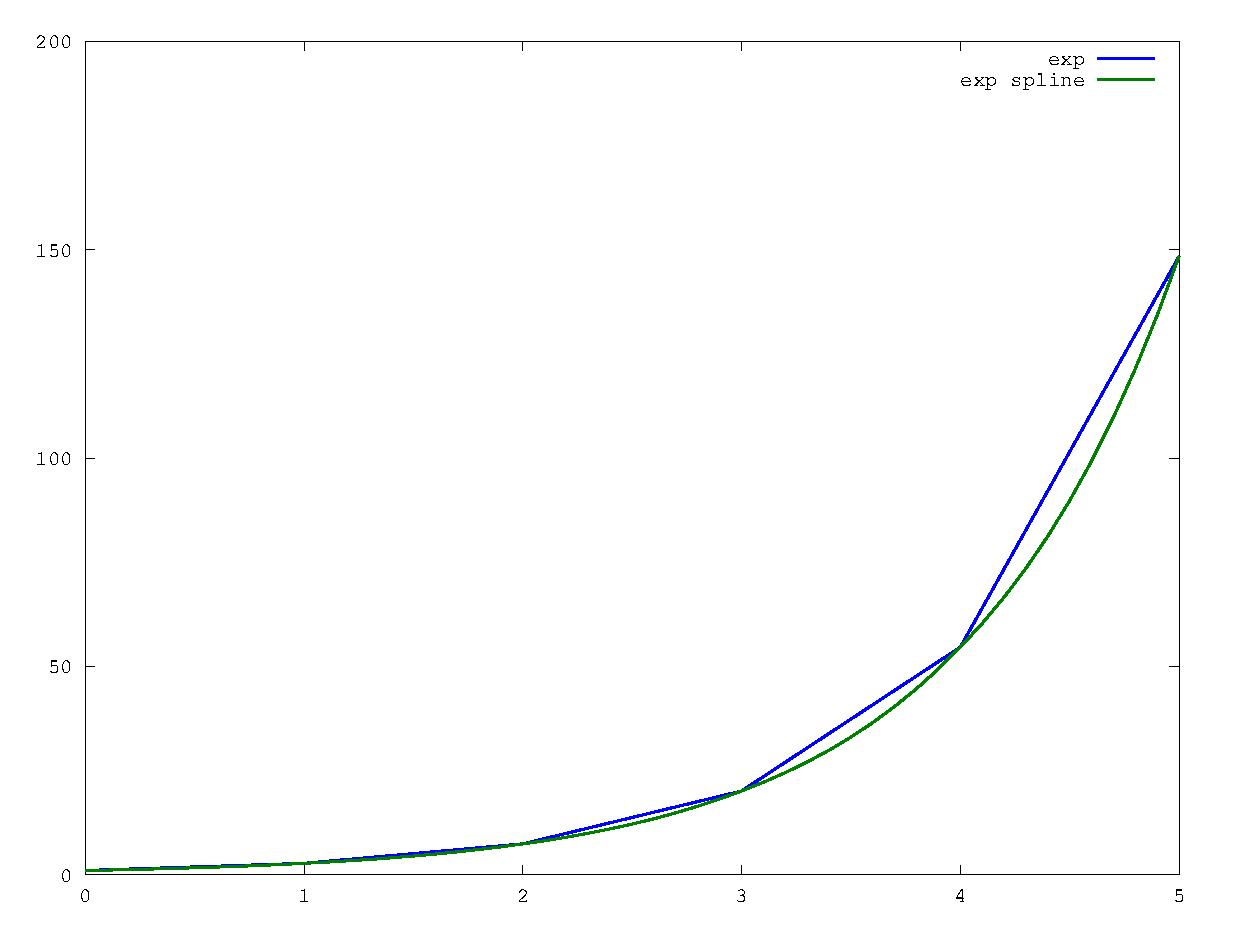
\includegraphics[scale=0.35]{../exp_10}    }
    \subfigure[Erreur interpolation.]{
      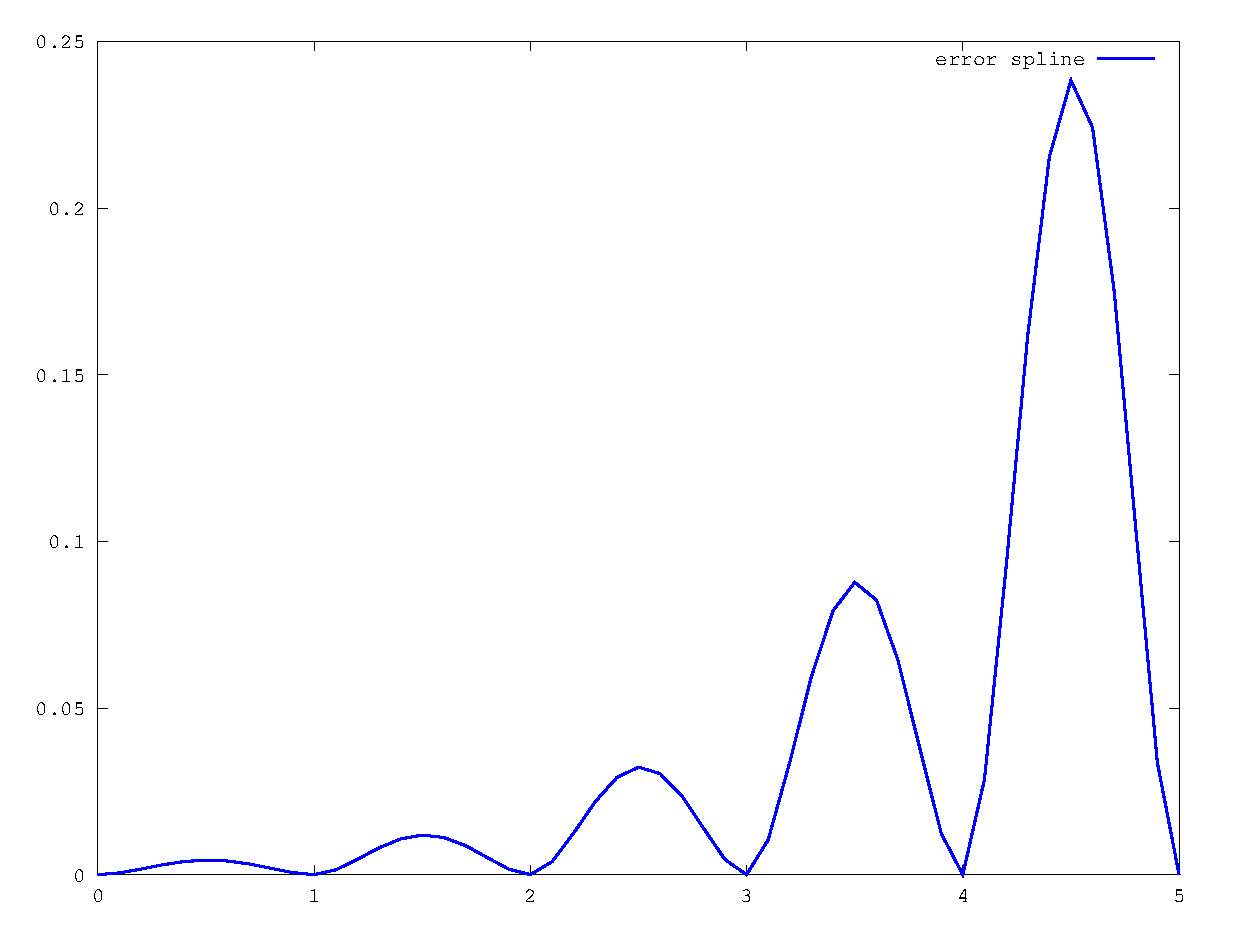
\includegraphics[scale=0.35]{../exp_10_error}
    }
    \par\end{centering}
  \caption{Fonction exp pas original 1, pas spline 0.1}
  \label{rspro}
\end{figure}


\begin{figure}[h!]
  \begin{centering}
    \subfigure[Interpolation]{
      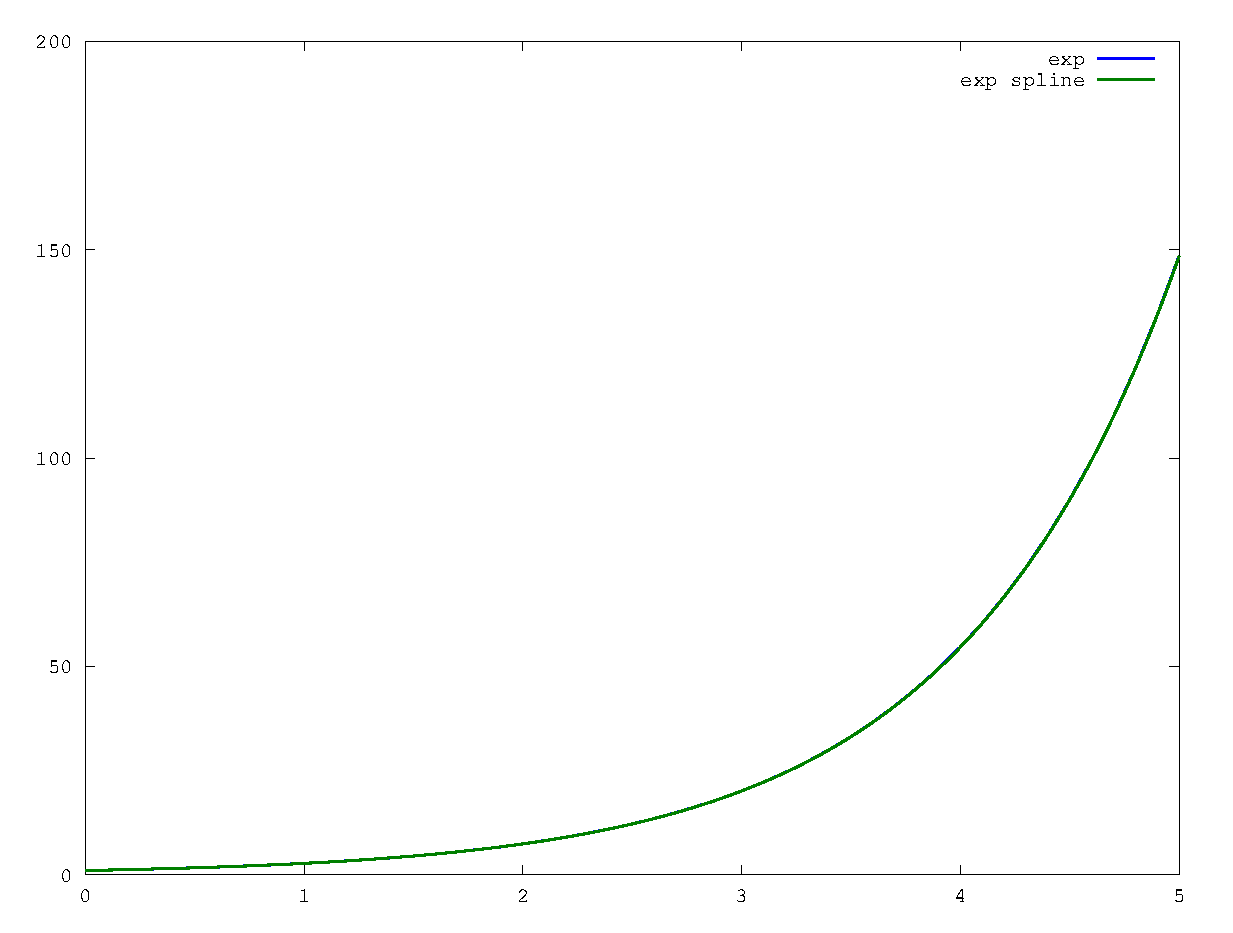
\includegraphics[scale=0.35]{../exp_10_2}    }
    \subfigure[Erreur interpolation.]{
      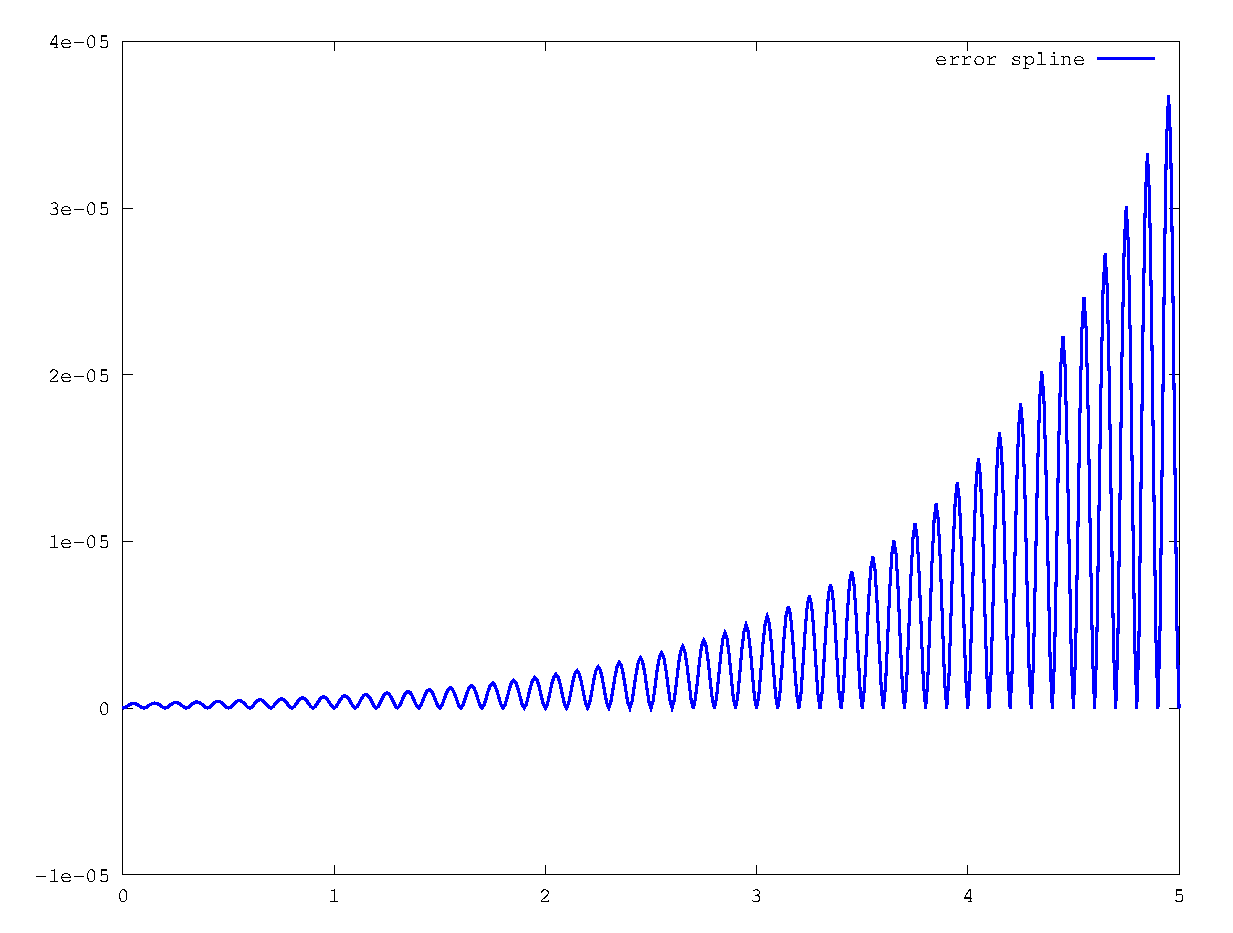
\includegraphics[scale=0.35]{../exp_10_error_2}
    }
    \par\end{centering}
  \caption{Fonction exp pas original 0.1, pas spline 0.01}
  \label{rspro}
\end{figure}

\end{document}

